\documentclass[tikz,border=5mm]{standalone}
\usepackage[T1]{fontenc}
\usepackage{helvet}
\renewcommand{\familydefault}{\sfdefault}
\usetikzlibrary{arrows.meta,positioning,fit,backgrounds,shapes.geometric}

\begin{document}
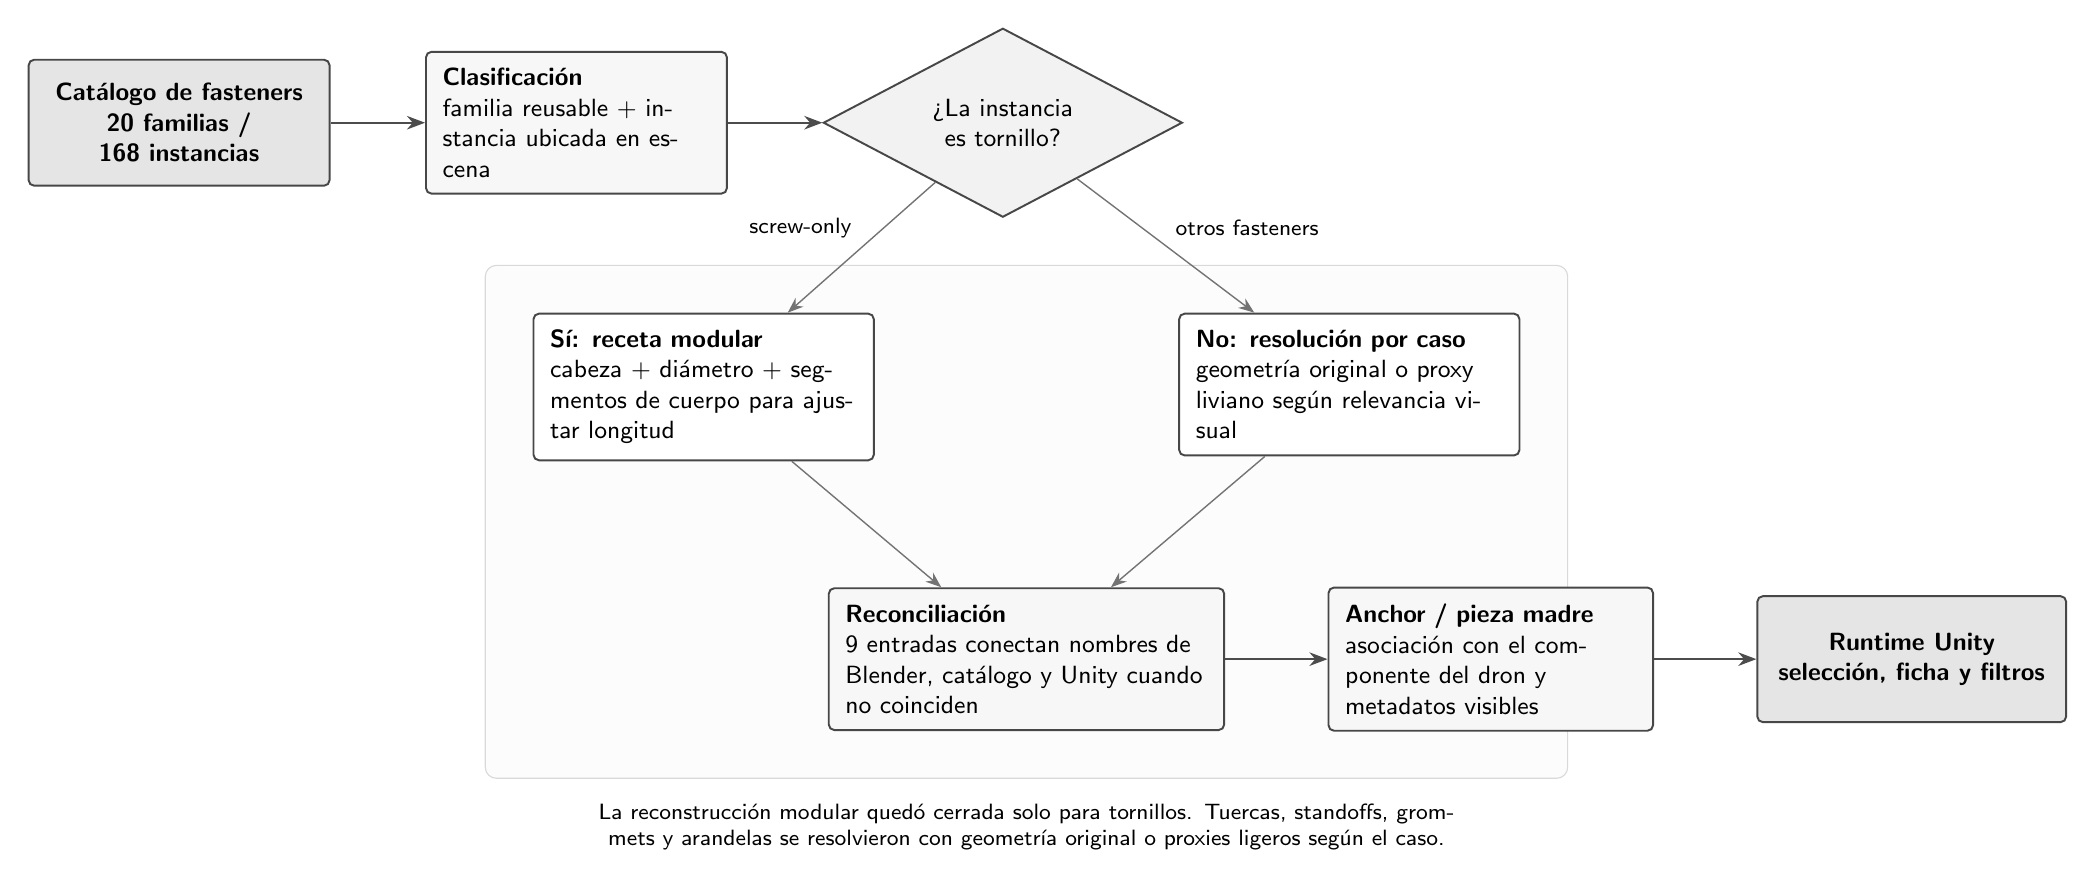
\begin{tikzpicture}[
  font=\sffamily\small,
  node distance=9mm and 12mm,
  box/.style={
    draw=black!72,
    rounded corners=2pt,
    line width=0.7pt,
    fill=black!3,
    align=left,
    text width=34mm,
    inner sep=6pt,
    minimum height=16mm
  },
  head/.style={box, fill=black!10, font=\sffamily\bfseries\small, align=center},
  decision/.style={
    diamond,
    aspect=1.9,
    draw=black!72,
    line width=0.7pt,
    fill=black!5,
    align=center,
    text width=30mm,
    inner sep=2pt
  },
  branch/.style={box, text width=39mm, fill=white},
  arrow/.style={-{Stealth[length=2.3mm]}, line width=0.65pt, draw=black!70},
  thin/.style={-{Stealth[length=2mm]}, line width=0.5pt, draw=black!55}
]

\node[head] (catalog) {Cat\'alogo de fasteners\\20 familias / 168 instancias};
\node[box, right=of catalog] (classify) {\textbf{Clasificaci\'on}\\familia reusable + instancia ubicada en escena};
\node[decision, right=of classify] (isScrew) {¿La instancia es tornillo?};

\node[branch, below=12mm of isScrew, xshift=-38mm] (screw) {\textbf{S\'i: receta modular}\\cabeza + di\'ametro + segmentos de cuerpo para ajustar longitud};
\node[branch, below=12mm of isScrew, xshift=44mm] (other) {\textbf{No: resoluci\'on por caso}\\geometr\'ia original o proxy liviano seg\'un relevancia visual};

\node[box, below=16mm of screw, xshift=41mm, text width=46mm] (reconcile) {\textbf{Reconciliaci\'on}\\9 entradas conectan nombres de Blender, cat\'alogo y Unity cuando no coinciden};
\node[box, right=13mm of reconcile, text width=37mm] (anchor) {\textbf{Anchor / pieza madre}\\asociaci\'on con el componente del dron y metadatos visibles};
\node[head, right=13mm of anchor, text width=35mm] (runtime) {Runtime Unity\\selecci\'on, ficha y filtros};

\draw[arrow] (catalog) -- (classify);
\draw[arrow] (classify) -- (isScrew);
\draw[thin] (isScrew) -- node[above left, font=\sffamily\footnotesize] {screw-only} (screw);
\draw[thin] (isScrew) -- node[above right, font=\sffamily\footnotesize] {otros fasteners} (other);
\draw[thin] (screw) -- (reconcile);
\draw[thin] (other) -- (reconcile);
\draw[arrow] (reconcile) -- (anchor);
\draw[arrow] (anchor) -- (runtime);

\begin{scope}[on background layer]
  \node[draw=black!15, rounded corners=4pt, fill=black!1,
    fit=(screw)(other)(reconcile),
    inner sep=6mm] {};
\end{scope}

\node[align=center, font=\sffamily\footnotesize, text width=125mm,
  below=8mm of reconcile] (note)
  {La reconstrucci\'on modular qued\'o cerrada solo para tornillos. Tuercas, standoffs, grommets y arandelas se resolvieron con geometr\'ia original o proxies ligeros seg\'un el caso.};

\end{tikzpicture}
\end{document}
